\chapter{Compilateur}
\begin{preamble}

\end{preamble}
\chpsummary{Contributions}
{
}
\section{Opérateurs}
%\begin{figure}[h]
\subsubsection*{Precedes(e$_1$,e$_2$):}
\begin{eplpseudocode}
$\llbracket$Precedes(e$_1$,e$_2$)$\rrbracket$=WindowIfComplex($\llbracket$e$_1$$\rrbracket$) $\rightarrow$ WindowIfComplex($\llbracket$e$_2$$\rrbracket$) and not WindowIfComplex($\llbracket$e$_1$$\rrbracket$) 
\end{eplpseudocode}
%\(Precedes(E_1,E_2)(t)=(\exists t_1)(\forall t_2)(E_1(t_1)\wedge E_2(t)\wedge (t_1<t)\wedge ((t_1<t_2\leq t)\rightarrow \thicksim E_1(t_2)\vee \thicksim E_2(t_2)))\)\\

\(Precedes(E_1,E_2)(t)=(\exists t_1)(\forall t_2)(E_1(t_1)\wedge \thicksim E_1(t) \wedge E_2(t)\wedge (t_1<t)\wedge ((t_1<t_2<t)\rightarrow \thicksim (E_1(t_2)\vee E_2(t_2))))\)\\

$Followed$-\(by(E_1,And\)-\(not(First(E_2),E_1))(t)\)

\(First(E_2)(t)=(\forall t_1)(E_2(t)\wedge ((t_1<t)\rightarrow \thicksim E_2(t_1)))\)

$And$-\(not(First(E_2),E_1)(t)=(\forall t_1)(\thicksim E_1(t)\wedge E_2(t)\wedge ((t_1<t)\rightarrow \thicksim (E_1(t_1)\vee E_2(t_1))))\)

$Followed$-\(by(E_1,And\)-\(not(First(E_2),E_1))(t)=(\exists t_1)(\forall t_2)(E_1(t_1)\wedge \thicksim E_1(t) \wedge E_2(t)\wedge (t_1<t)\wedge ((t_1<t_2<t)\rightarrow \thicksim (E_1(t_2)\vee E_2(t_2))))\)\\

\subsubsection*{During(e,s):}
\begin{eplpseudocode}
$\llbracket$During(e,s)$\rrbracket$=Becomes($\llbracket$s$\rrbracket$,v$_{sb}$) $\rightarrow$ ( every $\llbracket$e$\rrbracket$ ) and not Becomes($\llbracket$s$\rrbracket$,v$_{se}$)
\end{eplpseudocode}
\(During(E,E_{sb},E_{se})(t)=(\exists t_1)(\forall t_2)(E_{sb}(t_1)\wedge \thicksim E_{se}(t)\wedge E(t)\wedge (t_1<t)\wedge ((t_1<t_2< t)\rightarrow \thicksim E_{se}(t_2)))\)\\


$Followed$-\(by(E_{sb},And\)-\(not(Every(E),E_{se}))(t)\)

\(Every(E)(t)=E(T)\)

$And$-\(not(Every(E),E_{se})(t)=(\forall t_1)(\thicksim E_{se}(t)\wedge E(t)\wedge ((t_1<t)\rightarrow \thicksim (E_{se}(t_1)))\)

$Followed$-\(by(E_{sb},And\)-\(not(Every(E),E_{se}))(t)=(\exists t_1)(\forall t_2)(E_{sb}(t_1)\wedge \thicksim E_{se}(t)\wedge E(t)\wedge (t_1<t)\wedge ((t_1<t_2<t)\rightarrow \thicksim E_{se}(t_2)))\)\\

\subsubsection*{Overlapping(s$_1$,s$_2$):}
\begin{eplpseudocode}
$\llbracket$Overlapping(s$_1$,s$_2$)$\rrbracket$=Becomes($\llbracket$s$_1$$\rrbracket$,v$_{s_{1}b}$) $\rightarrow$ Becomes($\llbracket$s$_2$$\rrbracket$,v$_{s_{2}b}$) and not Becomes($\llbracket$s$_1$$\rrbracket$,v$_{s_{1}e}$)$ \rightarrow$ 
                                                Becomes($\llbracket$s$_1$$\rrbracket$,v$_{s_{1}e}$) and not Becomes($\llbracket$s$_2$$\rrbracket$,v$_{s_{2}e}$) 
\end{eplpseudocode}
\(Overlapping(E_{s_{1}b},E_{s_{1}e},E_{s_{2}b},E_{s_{2}e})(t)=(\exists t_1)(\exists t_2)(\forall t_3)(E_{s_{1}b}(t1)\wedge \thicksim E_{s_{1}e}(t_2)\wedge E_{s_{2}b}(t2)\wedge \thicksim E_{s_{2}e}(t) \wedge E_{s_{1}e}(t)\wedge (t_1<t_2<t)\wedge ((t_1<t_3\leq t_2)\rightarrow \thicksim E_{s_{1}e}(t_3)) \wedge ((t_2<t_3\leq t)\rightarrow \thicksim E_{s_{2}e}(t_3))) \)\\

\subsubsection*{Occurs(e,s):}
\begin{eplpseudocode}
$\llbracket$Occurs(e,s)$\rrbracket$=Becomes($\llbracket$s$\rrbracket$,v) $\rightarrow$ ( every-distinct(timestamp) $\llbracket$e$\rrbracket$ ) and not Becomes($\llbracket$s$\rrbracket$,v')
\end{eplpseudocode}
\(Occurs(E,E_{sb},E_{se})(t)=(\exists t_1)(\forall t_2)(E_{sb}(t_1)\wedge E(t)\wedge (t_1<t)\wedge ((t_1<t_2<t)\rightarrow \thicksim E_{se}(t_2) \vee \thicksim E(t_2)))\)\\

\subsubsection*{Occurs(s$_1$,s$_2$):}
\begin{eplpseudocode}
$\llbracket$Occurs(s$_1$,s$_2$)$\rrbracket$=((Becomes($\llbracket$s$_1$$\rrbracket$,v) $\rightarrow$ every-distinct(timestamp) Becomes($\llbracket$s$_2$$\rrbracket$,v) and not Becomes($\llbracket$s$_1$$\rrbracket$,v'))
                  or 
                  (Becomes($\llbracket$s$_2$$\rrbracket$,v) $\rightarrow$ every-distinct(timestamp) Becomes($\llbracket$s$_1$$\rrbracket$,v) and not Becomes($\llbracket$s$_2$$\rrbracket$,v')))
\end{eplpseudocode}
\begin{eplpseudocode}
$\llbracket$Occurs(s$_1$,s$_2$)$\rrbracket$=Occurs(Becomes($\llbracket$s$_2$$\rrbracket$,v),$\llbracket$s$_1\rrbracket$)
                 or 
                 Occurs(Becomes($\llbracket$s$_1$$\rrbracket$,v),$\llbracket$s$_2\rrbracket$)
\end{eplpseudocode}
\(Occurs(E_{s_{1}b},E_{s_{1}2},E_{s_{2}b},E_{s_{2}e})(t)=(\exists t_1)(\forall t_2)((E_{s_{1}b}(t_1)\wedge E_{s_{2}b}(t)\wedge ((t_1<t_2<t)\rightarrow \thicksim E_{s_{1}e}(t_2)) \wedge ((t_1<t_2<t)\rightarrow \thicksim E_{s_{2}b}(t_2)))\vee (E_{s_{2}b}(t_1)\wedge E_{s_{1}b}(t)\wedge ((t_1<t_2<t)\rightarrow \thicksim E_{s_{2}e}(t_2)) \wedge ((t_1<t_2<t)\rightarrow \thicksim E_{s_{1}b}(t_2)))  \wedge (t_1<t))\)\\

\(Occurs(E_{s_{1}b},E_{s_{1}e},E_{s_{2}b},E_{s_{2}e})(t)=Occurs(E_{s_{2}b},E_{s_{1}b},E_{s_{1}e})(t)\vee Occurs(E_{s_{1}b},E_{s_{2}b},E_{s_{2}e})(t) \)\\

\subsubsection*{And(e$_0$,$\dots$,e$_n$):}
\begin{eplpseudocode}
$\llbracket$And(e$_1$, $\dots$ ,e$_n$)$\rrbracket$=WindowIfComplex($\llbracket$e$_1$$\rrbracket$) and $\dots$ and WindowIfComplex($\llbracket$e$_n$$\rrbracket$)
\end{eplpseudocode}
\(And(E_1, \dots , E_n)(t)=(\exists t_{i=1;n})(\exists i_0)(\forall t')(E_1(t_1)\underset{i}\wedge E_i(t_i) \wedge E_n(t_n)\wedge (t_1\leq t)\underset{i}\wedge (t_i\leq t) \wedge (t_n\leq t)\wedge (t_{i_0}=t) \wedge ((t'<t)\rightarrow \thicksim E_{i_0}(t')))\)\\

\subsubsection*{Or(e$_0$,$\dots$,e$_n$):}
\begin{eplpseudocode}
$\llbracket$Or(e$_1$, $\dots$ ,e$_n$)$\rrbracket$=WindowIfComplex($\llbracket$e$_1$$\rrbracket$) or $\dots$ or WindowIfComplex($\llbracket$e$_n$$\rrbracket$)
\end{eplpseudocode}
\(Or(E_0, \dots , E_n)(t)=E_0(t)\vee \dots \vee E_n(t)\)

%\end{figure}
\subsubsection*{Followed-by}
``$\rightarrow$'' operator specifies that first the left hand expression must turn true and only then is the right hand expression evaluated for matching events.

$X\rightarrow Y$ because of CEP, $Y$ is the first event of its nature that succeeds to $X$.\\
\newline
$Followed$-\(by(E_1,E_2)(t)=(\exists t_1)(\forall t_2)(E_1(t_1)\wedge E_2(t)\wedge (t_1<t)\wedge ((t_1<t_2<t)\rightarrow \thicksim E_2(t_2)) )\)

\subsubsection*{not}
``$not$'' operator negates the truth value of an expression. Pattern expressions prefixed with ``$not$'' are automatically defaulted to true upon start, and turn permanantly false when the expression within thurns true. 

``$not$'' operator is generally used in conjuction with the ``$and$'' operator.

$X\ and\ not\ Y$ means that there must not have $Y$ events before $X$ event.\\
\newline
$And$-\(not(E_1,E_2)(t)=(\forall t_1)(\thicksim E_2(t)\wedge E_1(t)\wedge ((t_1<t)\rightarrow \thicksim E_2(t_1)))\)

\subsubsection*{every}
``$every$'' operator indicates that the pattern subexpression should restart when the subexpression qualified by the every keyword evaluates true or false.\\
\newline
\(Every(E)(t)=E(t)\)

\subsubsection*{first}

\(First(E)(t)=(\forall t_1)(E(t)\wedge ((t_1<t)\rightarrow \thicksim E(t_1)))\)


\section{Compilation vers pseudo-code EPL}
This section aim to describe generation of EPL pseudo-code from core DSL (in AST form).
EPL pseudo-code valid EPL operators. EPL does not support the notion of state, each state in a rule is translated into the corresponding events that marks the beginning and the end of the state.

\subsection{Abstract Syntax Tree}
\begin{center}
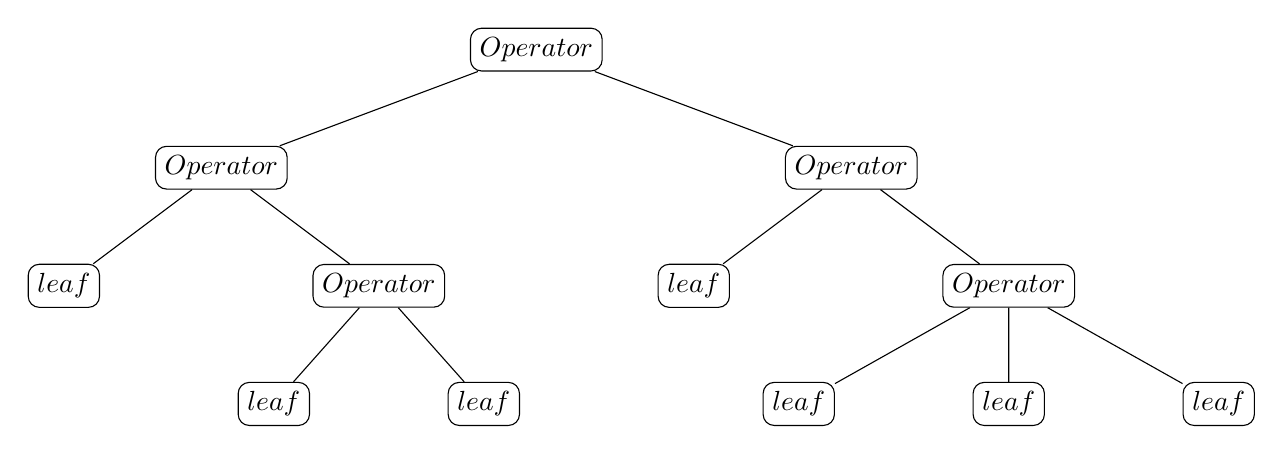
\begin{tikzpicture}[level/.style={sibling distance=80mm/#1},
  every node/.style = {shape=rectangle, rounded corners,
    draw, align=center}]]
  \node {$Operator$}
    child { node {$Operator$} 
      child { node {$leaf$}}
      child { node {$Operator$}
        child { node {$leaf$}}
        child { node {$leaf$}}}}
    child { node {$Operator$}
      child { node {$leaf$}}
      child { node {$Operator$}
        child { node {$leaf$}}
        child { node {$leaf$}}
        child { node {$leaf$}}}};
\end{tikzpicture}
\end{center}
\subsection*{Processing}
Post-Order traversal:\\
Traverse tree from bottom to top and from left to right. There is two main treatment, $leaf$ treatment and $operator$ treatment.
\begin{center}
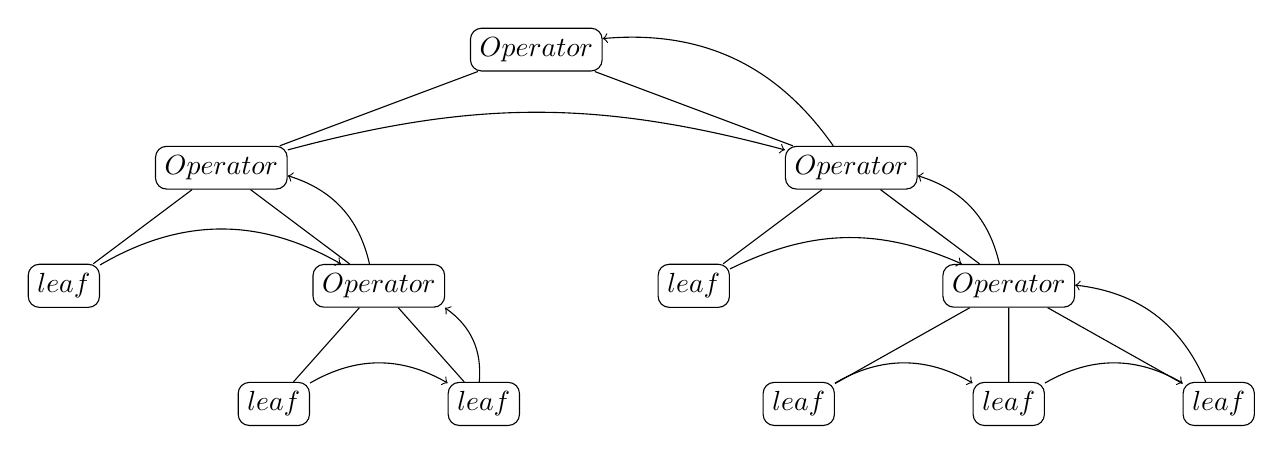
\begin{tikzpicture}[level/.style={sibling distance=80mm/#1},
  every node/.style = {shape=rectangle, rounded corners,
    draw, align=center}]]
  \node (n) {$Operator$}
    child { node (n0) {$Operator$} 
      child { node (n00) {$leaf$}}
      child { node (n01) {$Operator$}
        child { node (n010) {$leaf$}}
        child { node (n011) {$leaf$}}}}
    child { node (n1) {$Operator$}
      child { node (n10) {$leaf$}}
      child { node (n11) {$Operator$}
        child { node (n110) {$leaf$}}
        child { node (n111) {$leaf$}}
        child { node (n112) {$leaf$}}}};
\draw [->] (n00) edge[bend left]  (n01);
\draw [->] (n010) edge[bend left]  (n011);
\draw [->] (n011) edge[bend right=30,looseness=1]  (n01);
\draw [->] (n01) edge[bend right=30,looseness=1]  (n0);
\draw [->] (n0) edge[bend left=15]  (n1);
\draw [->] (n10) edge[bend left=25]  (n11);
\draw [->] (n110) edge[bend left]  (n111);
\draw [->] (n111) edge[bend left]  (n112);
\draw [->] (n112) edge[bend right=30,looseness=1]  (n11);
\draw [->] (n11) edge[bend right=30,looseness=1]  (n1);
\draw [->] (n1) edge[bend right=30,looseness=1]  (n);
\end{tikzpicture}
\end{center}
\subsection{Node}
Nodes in the AST concerns operators (except leaves).
In the AST a node has two attributes.
\begin{itemize}
\item operator's name 
\item code
\end{itemize}
\begin{center}
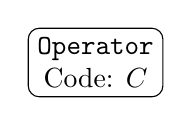
\begin{tikzpicture}[level/.style={sibling distance=80mm/#1},
  every node/.style = {shape=rectangle, rounded corners,
    draw, align=center}]]
  \node (n) {{\tt Operator}\\Code: $C$};
\end{tikzpicture}
\end{center}

\subsection{Atomic Events: Leaf}
Leaf are specialized nodes who can be state or event. All other nodes are only events.
\subsection*{Event}
{\tt e: p {\bf becomes} v $\Leftrightarrow p \Rightarrow v$ }\\ 
%The moment when an interaction or a sensor has a value change. Might concerns leaves and operators.
\subsection*{State}
{\tt s: p {\bf is} v $\Leftrightarrow p=v$ }\\
%A period in which an interaction or a sensor remains at a value, it has a beginning and an end.\\
Always concerns leaves.

Leaves are at the lowest level in the tree. It corresponds to the events or states expressed in the rules.
\begin{itemize}
\item raw sensors (Physical or Logical sensors):\\
event or state.
\begin{center}
\begin{tikzpicture}[level/.style={sibling distance=60mm/#1},
  every node/.style = {shape=rectangle, rounded corners,
    draw, align=center}]]
  \node (event) {{\tt e}\\Code: $e$};
  \node (state)[right=of event] {{\tt s}\\Code: $s$};
\end{tikzpicture}
\end{center}
\item sensor with filter $\mathds{S}\rightarrow \mathds{E}$:\\
\begin{center}
\begin{tikzpicture}[level/.style={sibling distance=40mm/#1},
  every node/.style = {shape=rectangle, rounded corners,
    draw, align=center}]]
  \node (less) {{\tt (s)\_delta(< time)}\\Code: {\it Becomes(s,v) $\rightarrow$ Becomes(s,v') where timer:within(time)}};
  \node (greater)[below=of less] {{\tt (s)\_delta(> time)}\\Code: {\it Becomes(s,v) $\rightarrow$ timer:interval(time) and not Becomes(s,v')}};
\end{tikzpicture}
\end{center}
\end{itemize}

The pseudo-code resulting of this step, for each operator, is stored in $Code$ attribute of the node.
\subsection{Complex Events: Functions}
This table show specificities of our defined operator in the compilation process.
\begin{figure}[h]
  \begin{tabular}{|l|c|c||c|} 
    \cline{1-4}
    \textbf{Kinds of operators}&\textbf{One generated rule} & \textbf{Alternative rules} & \textbf{Windowing state}\\
    \cline{1-4}
    Precedes \quad\quad\quad\quad$\mathds{E}\times\mathds{E}\rightarrow \mathds{E}$ & $\times$ &  & na\\
    \cline{1-4}
    During \quad\quad\quad\quad\quad$\mathds{E}\times\mathds{S}\rightarrow \mathds{E}$& $\times$ &  & $\times$ \\
    \cline{1-4} 
    Overlapping \quad\quad\quad$\mathds{S}\times\mathds{S}\rightarrow \mathds{E}$ & $\times$ &  & na\\
    \cline{1-4}
    Occurs \quad\quad\quad\quad\quad $\mathds{E}\times\mathds{S}\rightarrow \mathds{E}$& $\times$ &  & $\times$ \\
    \cline{2-4}
    \quad\quad\quad\quad\quad\quad\quad\quad$\ \mathds{S}\times\mathds{S}\rightarrow \mathds{E}$&  & $\times$ & na \\
    \cline{1-4}  
    And \quad\quad\quad $\ \mathds{E}\times\dots\times\mathds{E}\rightarrow \mathds{E}$& $\times$ & & na\\   
    % \cline{2-4} 
    % \quad$\{\mathds{E}\times\dots\times\mathds{E}\times\mathds{S}\}\times\mathds{S}\rightarrow \mathds{E}$&  & $\times$ & na \\ 
    \cline{1-4}
    Or \quad\quad\quad\quad$ \mathds{E}\times\dots\times\mathds{E}\rightarrow \mathds{E}$& $\times$  &  & na\\  
    \cline{1-4}
  \end{tabular}
  \caption{}
  \label{}
\end{figure}
\paragraph{One generated rule:} The funtion generates one rule to reconize the sequence of events.
\paragraph{Alternative rules:} The function generates more than one sequence of event to trigger a result. Meaning that there is more than one rule as result of the compilation of the operator. Thus the result of the compilation of a such operator is the composition of all rules resulting linked by an $Or$ operator.
For example, assuming the rules resulting of the compilation are noted {\tt rule$_1$} and {\tt rule$_2$}, the code resulting is ``$(\ rule_1\ )\ or\ (\ rule_2\ )$''.
\begin{center}
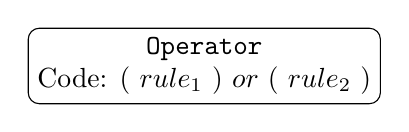
\begin{tikzpicture}[level/.style={sibling distance=80mm/#1},
  every node/.style = {shape=rectangle, rounded corners,
    draw, align=center}]]
  \node (n) {{\tt Operator}\\Code: $(\ rule_1\ )\ or\ (\ rule_2\ )$};
\end{tikzpicture}
\end{center}
\paragraph{Windowing state:} It means that the state in last state argument must cover all other arguments. Thus, all code of concerned son's node is brought back in their corresponding place in the sequence of events, instead of proceeding to a window creation.
\subsection{Intern functions}
Functions are used to generate EPL pseudo-code, especially extract beginning and end events from a state. 
\subsection*{Becomes: $\mathds{S}\times\mathds{B}\rightarrow \mathds{E}$}
This function translates a state into an event with the corresponding value.
\begin{lstlisting}[frame=single]
  $Becomes(p=v,v)\rightarrow p\Rightarrow v$
  $Becomes(p=v,v')\rightarrow p\Rightarrow v'$
\end{lstlisting}
\subsection*{WindowIfComplex}
This function checks if a window must be created and returns its id.
\begin{lstlisting}[frame=single]
  input: child
  output: window_id or leaf_code
  
  if child is leaf
  then
    return node's code
  else
    CreateWindow(child)
    return window_id
\end{lstlisting}

\subsection*{CreateWindow}
If a son of the current operator is a sequence of event, and the operator is not concerned by the covering of the last state, then a window is created to recognized this sub-sequence of events.
\begin{lstlisting}[frame=single]
input: node
output: window_id

create window window_id.std:unique(user,role.location) select * from StreamEvent
insert into window_id select rule_id from pattern [ TranstaleRule(code) ]
\end{lstlisting}
\paragraph{Optimization:} Because $Or$ operator has no priorities, each son with an $Or$ recognized by pattern matching, has its code bring back to the highest $Or$ operator code.
\section{Compilation vers EPL}
Once the tree has been traversed and all operators of each nodes has been processed, the last node's attributes code contains the final EPL pseudo-code rule
 
The final step is to obtain EPL form from final EPL pseudo-code rule, by completely instantiating the events.
To do so the form $name\Rightarrow value$ is converted using information provided by sensors stream static table.
\subsubsection*{TranslateRule}
\begin{lstlisting}[frame=single]
"name":{
  "location": "loc",
  "kind": "kind",
  "values":["val1","val2"]
}
\end{lstlisting}

\begin{lstlisting}[frame=single]
input: EPL pseudo-code // $name\Rightarrow val1$
output: EPL code // $name=StreamEvent(role.location=$`$loc$'$,role.kind=$`$kind$'$,value=$`$val1$'$)$
\end{lstlisting}
Moreover, this step binds all events in an EPL formula as originating from the same home, or specifying a specific home. 
Also, because of the recurring nature of rule this step introduce ``every'', at the beginning of the rule, to deal with multiple occurrences.
